\clearpage
\appendix
\pagestyle{addenda}
\renewcommand{\chaptername}{Appendix}
\chapter{Detailed Diagrams}
\label{sec:appendix_diagrams}

\noindent
This appendix presents the high-resolution, full-page versions of the diagrams discussed in previous chapters. These enlarged figures are provided to ensure optimal readability and to allow for a detailed inspection of the System's components, deployment nodes, and sequence logic.
Here is a summary of the diagrams included in this appendix.

\begin{table}[ht]
    \sf
    \small
    \centering
    \renewcommand{\arraystretch}{1.5}
    \begin{tabularx}{\textwidth}{|l|X|r|}
        \hline
        \rowcolor{lightgray} \textbf{Image} & \textbf{Description} & \textbf{Original Figure} \\
        \hline
        \textbf{\Cref{fig:appendix_component_diagram}} & UML component diagram & \Cref{fig:component_diagram} \\
        \textbf{\Cref{fig:appendix_deployment_diagram}} & Deployment view & \Cref{fig:deployment_diagram} \\
        \textbf{\Crefrange{fig:appendix_sd1_1}{fig:appendix_sd1_2}} & SD1 sequence: Sign Up by a User & \Cref{fig:SD1} \\
        \textbf{\Cref{fig:appendix_sd2}} & SD2 sequence: Log In by a User & \Cref{fig:SD2} \\
        \textbf{\Cref{fig:appendix_sd3}} & SD3 sequence: Access as Guest & \Cref{fig:SD3} \\
        \textbf{\Crefrange{fig:appendix_sd4_1}{fig:appendix_sd4_2}} & SD4 sequence: Record a Trip & \Cref{fig:SD4} \\
        \textbf{\Cref{fig:appendix_sd5}} & SD5 sequence: Validate a Trip and a Path & \Cref{fig:SD5} \\
        \textbf{\Cref{fig:appendix_sd6}} & SD6 sequence: Change Path's Visibility & \Cref{fig:SD6} \\
        \textbf{\Crefrange{fig:appendix_sd7_1}{fig:appendix_sd7_2}} & SD7 sequence: Create a Path Manually & \Cref{fig:SD7} \\
        \textbf{\Cref{fig:appendix_sd8}} & SD8 sequence: Search for a Route & \Cref{fig:SD8} \\
        \textbf{\Cref{fig:appendix_sd9}} & SD9 sequence: Delete a Trip & \Cref{fig:SD9} \\
        \textbf{\Cref{fig:appendix_sd10}} & SD10 sequence: Delete a Path & \Cref{fig:SD10} \\
        \hline
    \end{tabularx}
    \caption{Reference table for detailed diagrams in the appendix}
\end{table}

\begin{sidewaysfigure}[hp]
    \centering
    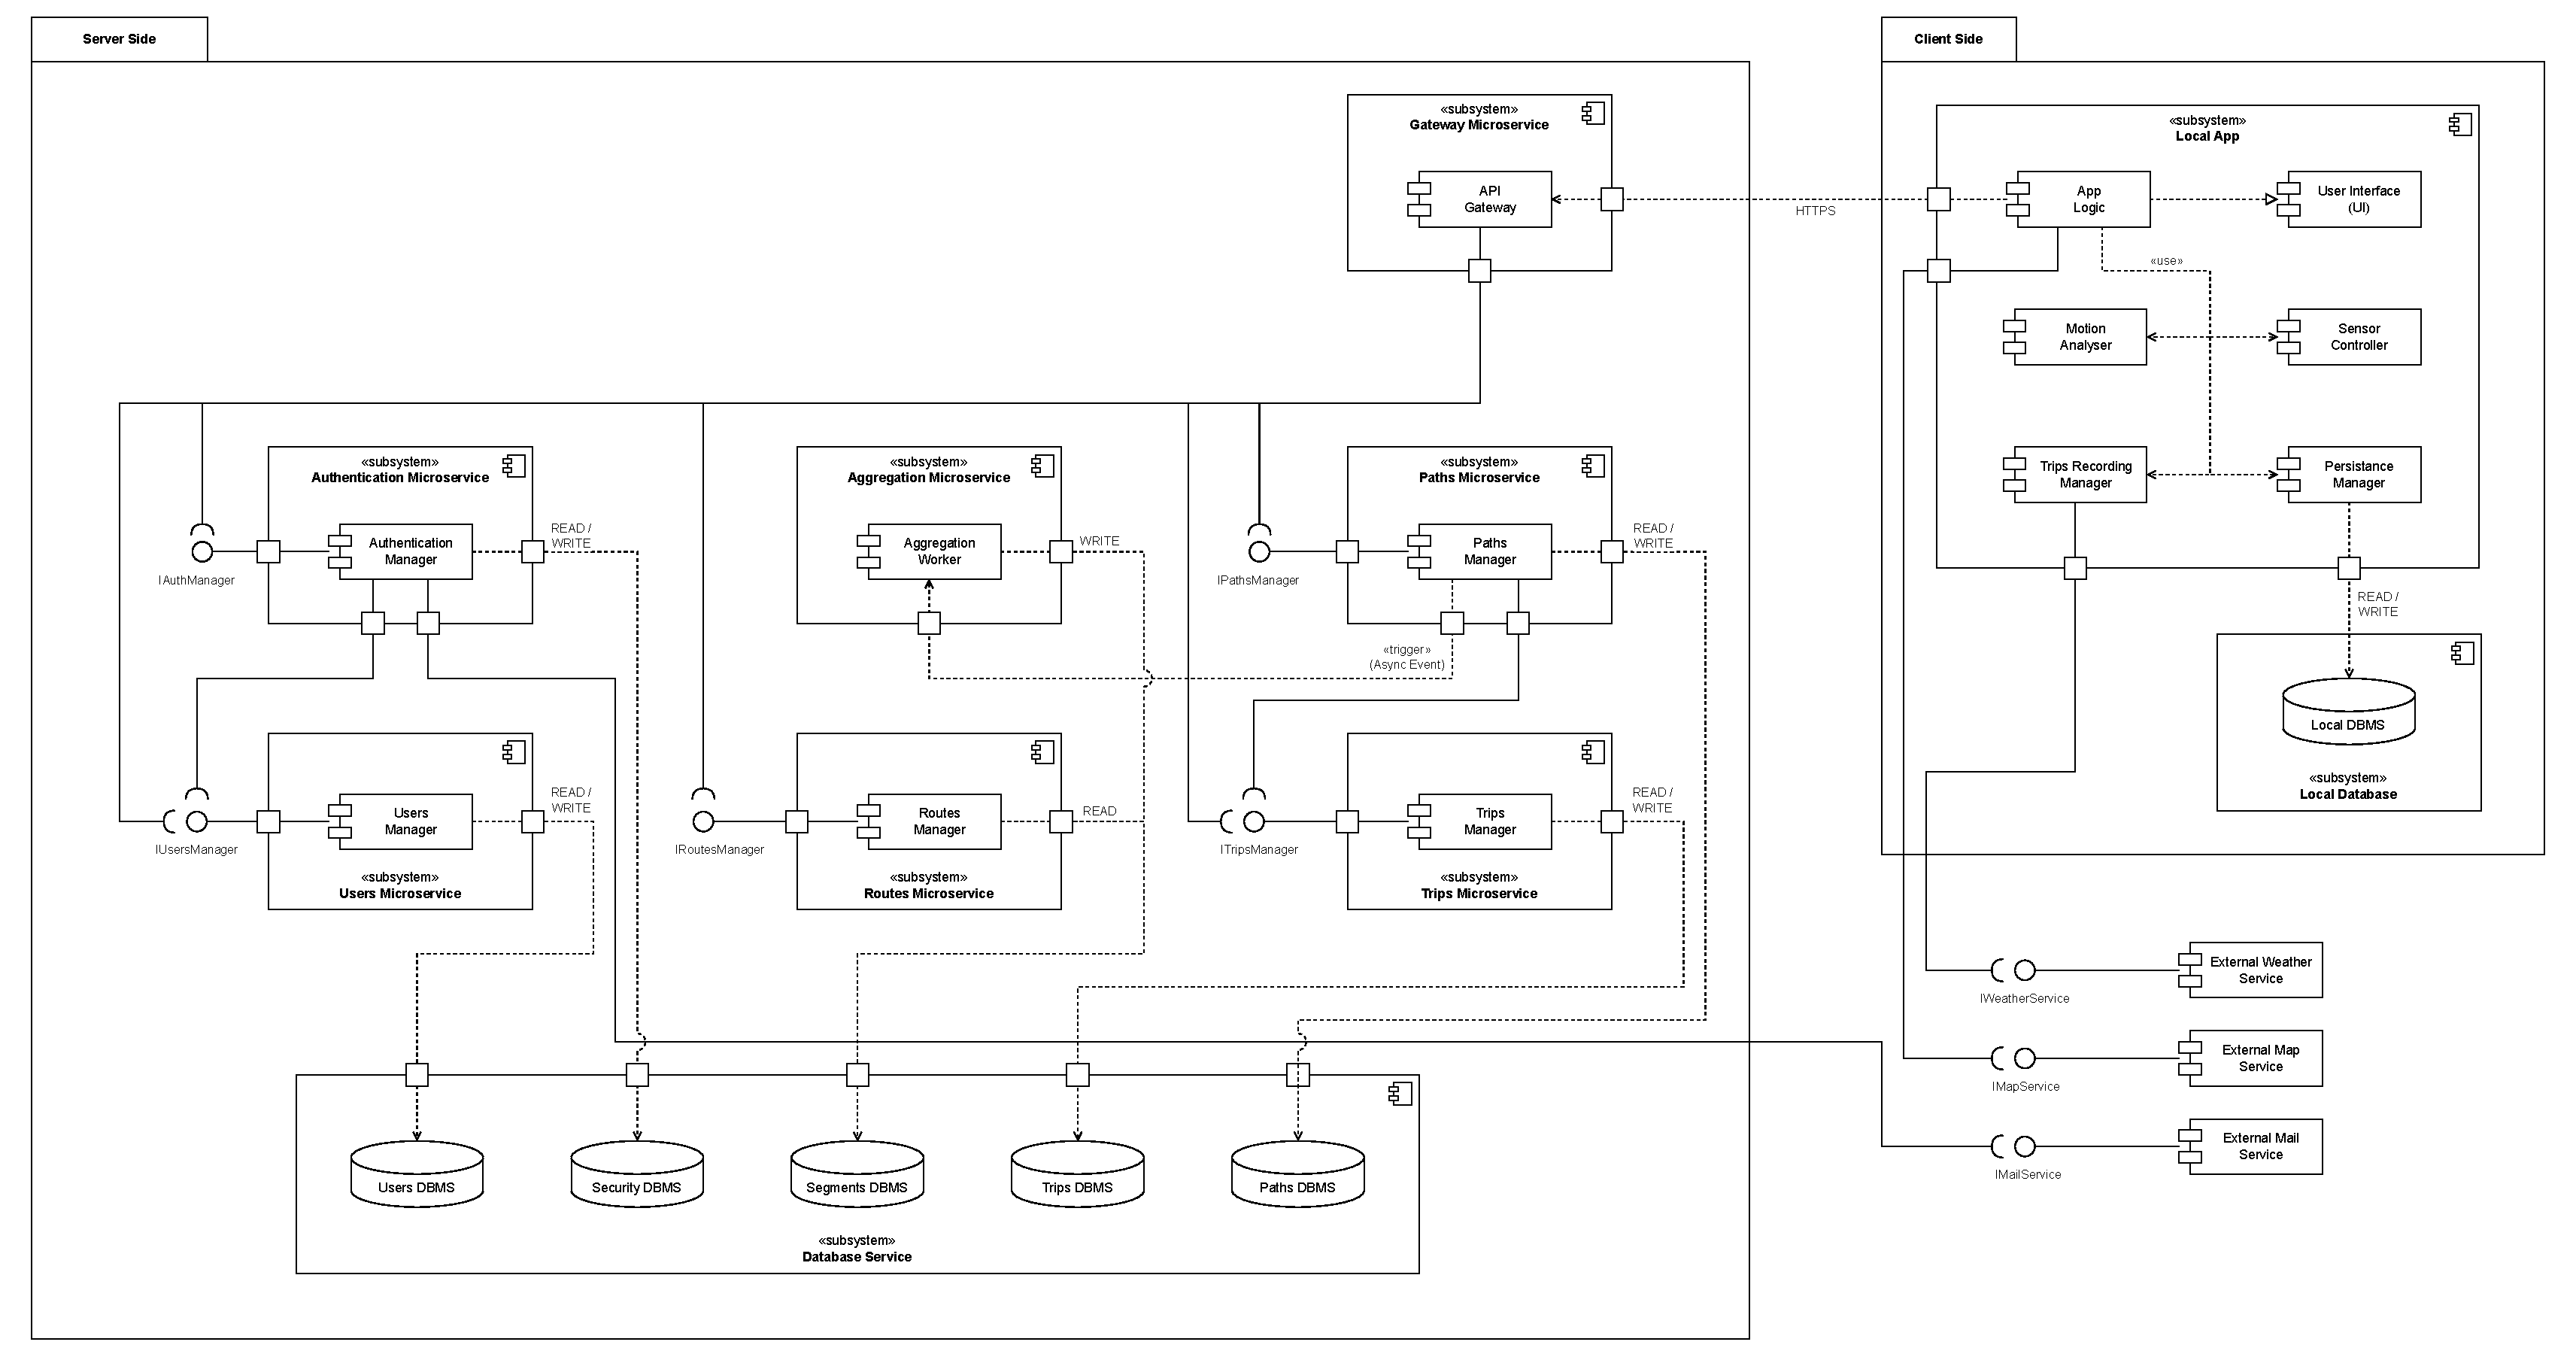
\includegraphics[width=\textwidth]{pdf/component_diagram.pdf}
    \caption{Full page UML Components Diagram.}
    \label{fig:appendix_component_diagram}
\end{sidewaysfigure}


\begin{sidewaysfigure}[hp]
    \centering
    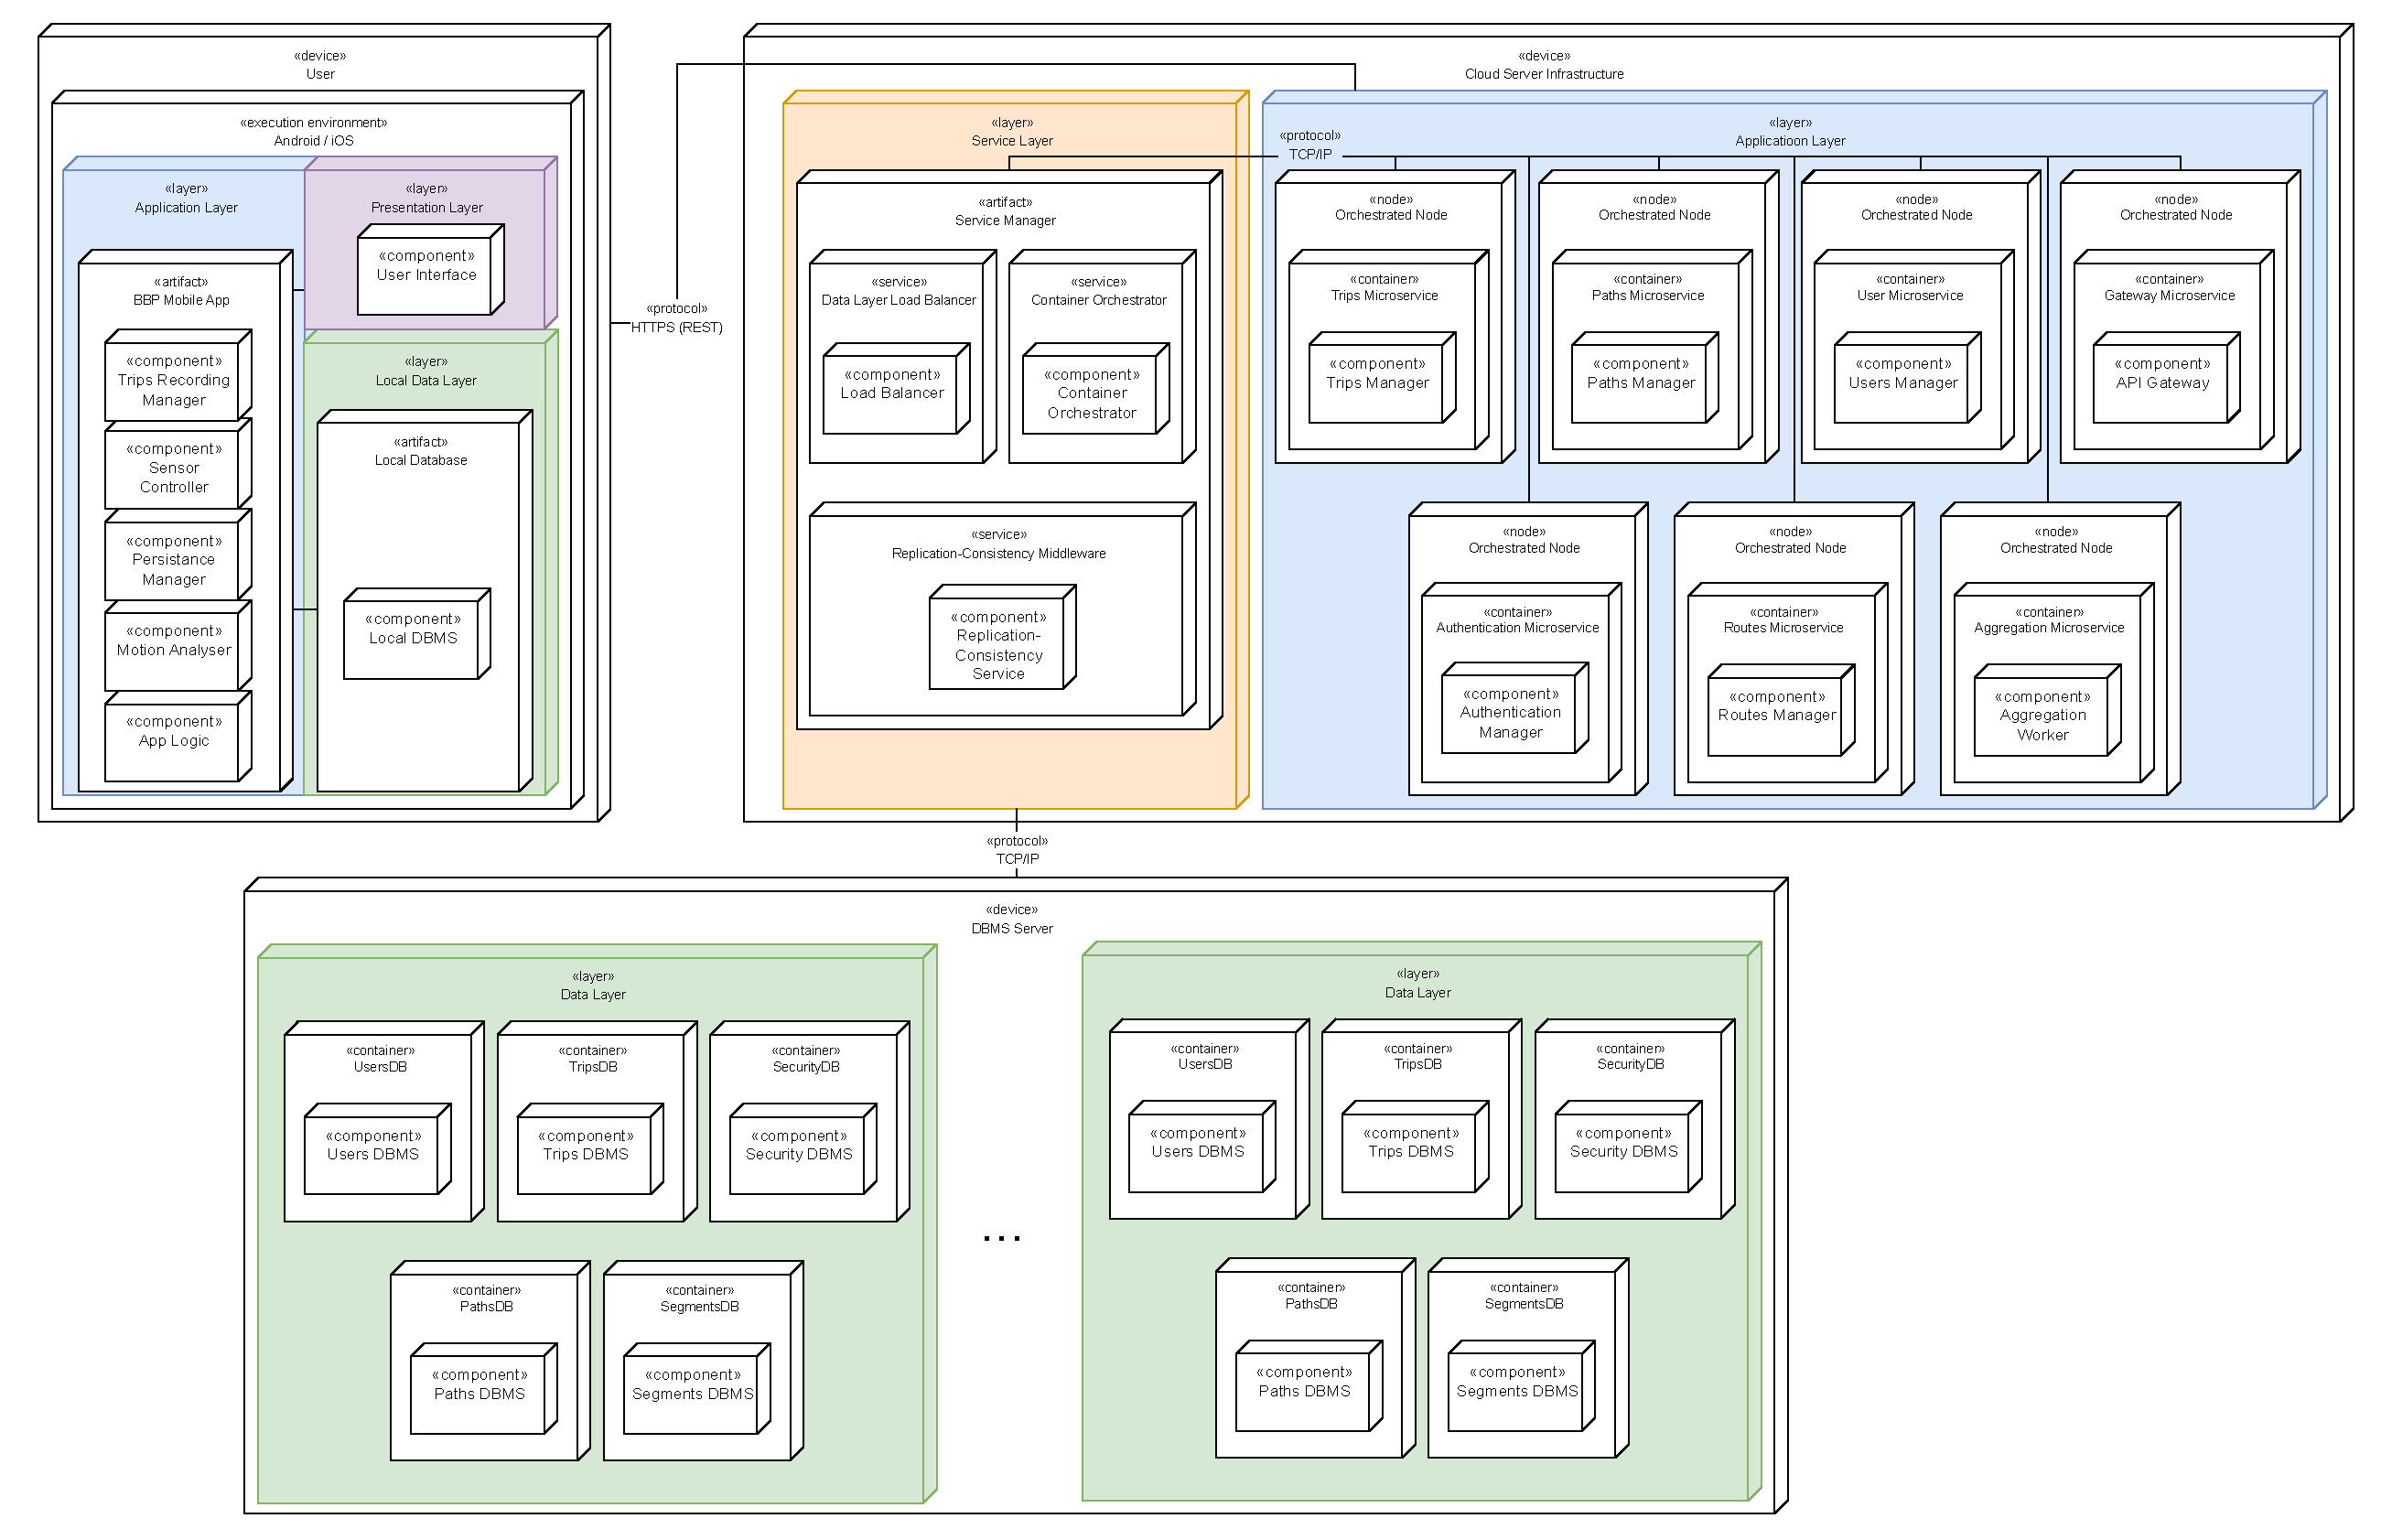
\includegraphics[width=\textwidth, keepaspectratio]{pdf/deployment_diagram.pdf}
    \caption{Full page Deployment View of Best Bike Paths System}
    \label{fig:appendix_deployment_diagram}
\end{sidewaysfigure}

\begin{sidewaysfigure}[hp]
    \centering
    \includesvg[width=0.9\textwidth, keepaspectratio, inkscapelatex=false]{figures/sd1_part1.svg}
    \caption{SD1. Full page diagram (part 1)}
    \label{fig:appendix_sd1_1}
\end{sidewaysfigure}

\begin{sidewaysfigure}[hp]
    \centering
    \includesvg[width=0.9\textwidth, keepaspectratio, inkscapelatex=false]{figures/sd1_part2.svg}
    \caption{SD1. Full page diagram (part 2)}
    \label{fig:appendix_sd1_2}
\end{sidewaysfigure}

\begin{sidewaysfigure}[hp]
    \centering
    \includesvg[width=0.75\textwidth, keepaspectratio, inkscapelatex=false]{figures/sd2.svg}
    \caption{SD2. Full page diagram}
    \label{fig:appendix_sd2}
\end{sidewaysfigure}

\begin{sidewaysfigure}[hp]
    \centering
    \includesvg[width=\textwidth, keepaspectratio, inkscapelatex=false]{figures/sd3.svg}
    \caption{SD3. Full page diagram}
    \label{fig:appendix_sd3}
\end{sidewaysfigure}

\begin{sidewaysfigure}[hp]
    \centering
    \includesvg[width=0.75\textwidth, keepaspectratio, inkscapelatex=false]{figures/sd4_part1.svg}
    \caption{SD4. Full page diagram (part 1)}
    \label{fig:appendix_sd4_1}
\end{sidewaysfigure}

\begin{sidewaysfigure}[hp]
    \centering
    \includesvg[width=0.9\textwidth, keepaspectratio, inkscapelatex=false]{figures/sd4_part2.svg}
    \caption{SD4. Full page diagram (part 2)}
    \label{fig:appendix_sd4_2}
\end{sidewaysfigure}

\begin{sidewaysfigure}[hp]
    \centering
    \includesvg[width=0.9\textwidth, keepaspectratio, inkscapelatex=false]{figures/sd5.svg}
    \caption{SD5. Full page diagram}
    \label{fig:appendix_sd5}
\end{sidewaysfigure}

\begin{sidewaysfigure}[hp]
    \centering
    \includesvg[width=0.8\textwidth, keepaspectratio, inkscapelatex=false]{figures/sd6.svg}
    \caption{SD6. Full page diagram}
    \label{fig:appendix_sd6}
\end{sidewaysfigure}

\begin{sidewaysfigure}[hp]
    \centering
    \includesvg[width=0.9\textwidth, keepaspectratio, inkscapelatex=false]{figures/sd7_part1.svg}
    \caption{SD7. Full page diagram (part 1)}
    \label{fig:appendix_sd7_1}
\end{sidewaysfigure}

\begin{sidewaysfigure}[hp]
    \centering
    \includesvg[width=\textwidth, keepaspectratio, inkscapelatex=false]{figures/sd7_part2.svg}
    \caption{SD7. Full page diagram (part 2)}
    \label{fig:appendix_sd7_2}
\end{sidewaysfigure}

\begin{sidewaysfigure}[hp]
    \centering
    \includesvg[width=\textwidth, keepaspectratio, inkscapelatex=false]{figures/sd8.svg}
    \caption{SD8. Full page diagram}
    \label{fig:appendix_sd8}
\end{sidewaysfigure}

\begin{sidewaysfigure}[hp]
    \centering
    \includesvg[width=0.95\textwidth, keepaspectratio, inkscapelatex=false]{figures/sd9.svg}
    \caption{SD9. Full page diagram}
    \label{fig:appendix_sd9}
\end{sidewaysfigure}

\begin{sidewaysfigure}[hp]
    \centering
    \includesvg[width=0.9\textwidth, keepaspectratio, inkscapelatex=false]{figures/sd10.svg}
    \caption{SD10. Full page diagram}
    \label{fig:appendix_sd10}
\end{sidewaysfigure}